%!TEX program = xelatex
\documentclass[a4paper,11pt]{article}
\usepackage{hyperref}
\hypersetup{
		colorlinks = true,
    	linkcolor = blue,
    	citecolor = blue,
    	linktoc=all
}
\usepackage{graphicx}
\usepackage[utf8]{inputenc}
\usepackage[T1]{fontenc}
\usepackage[francais]{babel}
\usepackage[dvipsnames]{xcolor}
\usepackage{hyphenat}
\usepackage{datetime}
\usepackage{wrapfig}
\usepackage[top=3cm, bottom=3cm, left=2.5cm, right=2.5cm]{geometry}
\usepackage{url}
\usepackage{caption}
\usepackage{subcaption}
\usepackage{listings}
\usepackage{wrapfig}
\usepackage{lipsum}
\usepackage{titlesec}
\setcounter{secnumdepth}{4}
\lstset{frame=tb,
  language=C,
  aboveskip=3mm,
  belowskip=3mm,
  showstringspaces=false,
  columns=flexible,
  basicstyle={\small\ttfamily},
  numbers=none,
  %numberstyle=\color{RedOrange},
  %keywordstyle=\color{blue},
  %commentstyle=\color{OliveGreen},
  breaklines=true,
  breakatwhitespace=true,
  tabsize=4
}



\begin{document}

	\sloppy
	\fontsize{12pt}{18pt}\selectfont
	\begin{figure}[htbp]
		\begin{minipage}[b]{0.5\linewidth}
			\centering
			
\includegraphics[width=\linewidth]{pictures/worldline.jpg}
		\end{minipage}
		\hspace{3cm}
		\begin{minipage}[b]{0.25\linewidth}
			\centering
			
\includegraphics[width=\linewidth]{pictures/telecom.png}
		\end{minipage}
	\end{figure}

	\begin{center}
	\textbf{\Large{Télécom ParisTech \\
			Promotion 2017 \\
			Sylvain DASSIER}}
	
	\end{center}


	\vspace{2cm}
	\begin{center}
		\huge{\textbf{RAPPORT DE STAGE}} \\
		\vspace{1cm}
		\textbf{%
		\textcolor{blue}{Étude de l'apport du protocol MPTCP dans l'optimisation du trafic}} \\
		
	\end{center}



	\vspace{1cm}
	
		\textbf{
			\begin{tabbing}
		  		Département : ~~~~~~~~\= \textit{Département d'Informatique} \\
		 	 	Option : \> \textit{INFRES} \\
		  		Encadrants : \> \textit{M. Luigi IANNONE, M. Antoine FRESSANCOURT} \\
		  		Dates : \> \textit{18/07/2016 - 17/01/2017} \\
		 		Adresse : \> \textit{Télécom ParisTech, 23 Avenue d'Italie,} \\
		  				\> \textit{75013 Paris}
			\end{tabbing}
		}
		
	\clearpage
	
	\begin{center}
		\Huge{\textbf{Declaration d'intégrité relative au plagiat}}
	\end{center}
	\vspace{3cm}
	\emph{Je soussigné} DASSIER Sylvain \emph{certifie sur l'honneur :}\\
	\begin{enumerate}
	  	\item Que les résultats décrits dans ce rapport sont l'aboutissement de mon
	  	travail.
		\item Que je suis l'auteur de ce rapport.
		\item Que je n'ai pas utilisé des sources ou résultats tiers sans
		clairement les citer et les référencer selon les règles bibliographiques
		préconisées.
	\end{enumerate}
	\vspace{2cm}
	
\includegraphics[scale=0.3]{pictures/declaration.jpg}
	
	\vspace{-1cm}
	\formatdate{17}{01}{2017}
	\hspace{5cm}
	Signature : 
\includegraphics[scale=0.5]{pictures/signa.jpg}
	
	\clearpage


	\section*{\Huge \textcolor{blue}{\textit{Abstract}}}
	
		\begin{description}
		
			\item \hspace{2cm} In urban developed areas characterised by sustainable economic growth and high quality of life, we have seen high levels of investment in the domain of vehicle to vehicle and vehicle to infrastructure technologies. CarFi is a project that deals with connected vehicles and allows them to take advantage of Wifi hotspots in addition to 2G, 3G or 4G to connect to the Internet while on the move. During this internship we have tried to look at the solutions provided by the MPTCP protocol in order to maintain perpetual connection to the Internet. A part of our work is dedicated to putting in place a debugging system for the better comprehension of the MPTCP protocol. We have particularly looked at the enhanced socket API for Multipath TCP developed by L'Université Catholique de Louvain. This API allows us to manipulate sub flows from the Application Layer. In fact, we have put in place a testbed with the application Netcat to verify the functioning of the API according to our needs. Finally we have tried to evaluate the performance of our developed netcat-mptcp.
			
		\end{description}
		
	\section*{\Huge \textcolor{blue}{\textit{Résumé}}}
	
		\begin{description}

			\item \hspace{2cm} Dans les villes urbaines et dévéloppées, caractérisées par une croissance économique stable et une qualité de vie élevée, nous avons constaté un grand nombre d'investissements dans le domaine des technologies véhicule à véhicule et véhicule à infrastructure. CarFi est un projet qui inclut les véhicules connectées et qui leur permet de profiter des avantages des hotspots Wifi en complément des réseaux 2G, 3G ou 4G pour se connecter à Internet en étant en mouvement. Pendant ce stage nous avons essayé de voir les solutions proposées par le protocol MPTCP pour maintenir une connexion internet perpetuelle. Une partie de notre travail est dédiée à la mis en place d'un système de déboggage pour mieux comprendre le protocol MPTCP. Nous avons en particulier regardé une API basée sur MPTCP et dévéloppée par l'Université Catholique de Louvain. L'API nous a permis de manipuler les sous flux de la couche application. Nous avons également mis en place un banc d'essai avec l'application Netcat pour vérifier le bon fonctionnement de l'API selon nos besoins. Par ailleurs, nous avons évalué la performance de notre solution proposée (netcat-mptcp).
			
		\end{description}
		
	

	\clearpage

	\setcounter{tocdepth}{3}

	\tableofcontents

	\clearpage

	
	\section{Introduction}

		\vspace{0.5cm}
		\subsection{Context}
			\begin{description}
				\item \hspace{2cm} Today, connected vehicles make use of 2G, 3G or 4G networks in order to connect to the Internet while in motion. Whether it be for GPS, simple browsing, emergency calls, e-calls or music, every consumer has his/her own needs. \\

				Apart from the usual connection glitches, such connectivity is rather expensive with limited bandwidth. Even though workarounds have been implemented, most of them are either inefficient or are not completely transparent. These limitations stand in the way of developement of connected vehicles. \\

				In fact, there has been a lot of research work in present times on vehicle to vehicle and vehicle to infrastructure technologies \cite[V2x]{V2I}. Car manufacturers and infrastructure suppliers are investing in such projects to keep up with the growing demand. However we are still waiting for a concrete outcome which is immediately deployable. Our project \textbf{CarFi} may play the role of an intermediary as something functional but which can be further developed with these vehicle to vehicle and vehicle to infrastructure technologies \cite[V2x]{V2x, smartcities}. \\

				MultiPath TCP (MPTCP) is an effort towards enabling the simultaneous use of several IP-addresses/interfaces by a modification of TCP. It presents a regular TCP interface to applications, while in fact spreading data across several sub-flows. Benefits of this include better resource utilisation, better throughput and smoother reaction to failures. The \textbf{CarFi} project aims to exploit these advantages of MPTCP. A potential add-on would be the usage of the WiFi network when available. Most urban areas are covered via Mobile Network Operator or ISP WiFi hotspots. One may envisage a scenario where the default connection is established over Wifi and when it is no longer available, the communication carries on over 3G. \\

				\textbf{Our Objective :} To develop a functional prototype for the \textbf{CarFi} project. This prototype is based on the \textbf{Enhanced Socket API for Multipath TCP} \cite[API]{api}. It ensures continuous connectivity to the network, keeping certain channels like the 3G as pivots/fallbacks and others like the Wifi to join and leave. It may also be used for optimum usage of network resources while using all the channels available.
				
			\end{description}
	
		\clearpage
		\subsection{Document Outline}
			\begin{description}
				\item \hspace{2cm} This document is divided into two main parts comprising different sections. The first part involves section \hyperref[sec:mptcpdebug]{2} where we describe how to set up a \textbf{\emph{debugging environment for MPTCP}}. This will help us to follow the different system calls during the establishment of a flow or a sub-flow. The next sections form the other part, dealing with the new socket API that enables us to control the MPTCP stack from user space. Section \hyperref[sec:mptcpapi]{3} gives a description of the socket API along with some details on its implementation. Section \hyperref[sec:netcat-mptcp]{4} elaborates a use case of this API, in our case a \textbf{Netcat} with \textbf{MPTCP}. Section \hyperref[sec:res]{5} summarises our results \hyperref[subsec:result]{5.1}, elucidates certain statistics \hyperref[subsec:statistics]{5.2} and mentions some of the underperformances and anomalies \hyperref[sec:furtherdevelopment]{7} encountered.
			\end{description}



	\vspace*{1.5cm}

	\begin{center}
		\LARGE\textbf{PART I}
	\end{center}


	\section{Setting up a debugging environment for MPTCP : }

		\label{sec:mptcpdebug}

		In order to understand the different stages of running of the MPTCP linux kernel, we have put in place a debugging environment. In fact, after doing a little bit of research, we have come across various methods for debugging a protocol. Solutions like \textbf{Eclipse + GDB}, \textbf{NS3 + DCE for in-kernel protocol implementation} \cite[NS3+DCE]{inkernel}, \textbf{net-next-nuse} \cite[net-next-nuse]{net-next-nuse} or \textbf{net-next-sim} \cite[net-next-sim]{net-next-sim} exist. In any case, all debugging systems involving a protocol implementation are very complex. \\

		We have chosen and succesfully implemented \cite[LibOS]{libos} (an MPTCP version of the library operating system of the linux kernel) with \cite[DCE]{dce} (Direct Code Execution). A library version of a protocol is faster and easier to compile and put in place, hence the choice. Everything was done on a XUbuntu 14.04 64bit virtual machine with DCE 1.8. During the setting up of the debugging system we received the valuable help from \textbf{M. Matthieu Coudron} of \textbf{L'Université Pierre-et-Marie-Curie}. The discussions can be found here : \cite[ns-3-dce]{ns-3-dce}. The following illustrates how to set up the debug environment :

		\begin{enumerate}
			
			\item \textbf{Install the dependencies :} \\Since we are doing everything on a virgin operating system, we need to install certain dependencies to make things work. These dependencies are essential for the different components of the debugging system viz. \textbf{NS3}, \textbf{DCE} etc. to run properly and collaborate with one another.
				
			\begin{lstlisting}
				sudo apt-get install vim git mercurial gcc g++ python python-dev qt4-dev-tools libqt4-dev bzr cmake libc6-dev libc6-dev-i386 g++-multilib gdb valgrind gsl-bin libgsl0-dev libgsl0ldbl flex bison libfl-dev tcpdump sqlite sqlite3 libsqlite3-dev libxml2 libxml2-dev libgtk2.0-0 libgtk2.0-dev vtun lxc uncrustify doxygen graphviz imagemagick texlive texlive-extra-utils texlive-latex-extra texlive-font-utils dvipng python-sphinx dia python-pygraphviz python-kiwi python-pygoocanvas libgoocanvas-dev ipython libboost-signals-dev libboost-filesystem-dev openmpi-bin openmpi-common openmpi-doc libopenmpi-dev libncurses5-dev libncursesw5-dev unrar unrar-free p7zip-full autoconf libpcap-dev cvs libssl-dev wireshark
			\end{lstlisting}

			\item \textbf{Build DCE using bake :} \\The easiest way to build \textbf{DCE} is to use \textbf{bake} \cite[bake]{bake}. It automates the building process by handling dependencies, downloading required sources, correctly building required modules, providing off-line installation and build capabilities and providing the possibility to configure according to one's needs.

				\begin{lstlisting}
					hg clone http://code.nsnam.org/bake bake
					export BAKE_HOME=`pwd`/bake
					export PATH=$PATH:$BAKE_HOME
					export PYTHONPATH=$PYTHONPATH:$BAKE_HOME
					mkdir dce
					cd dce
					bake.py configure -e dce-ns3-1.8
					bake.py download
					bake.py build
				\end{lstlisting}

			\item \textbf{Download and build the \emph{mptcp\_trunk\_libos} branch of \emph{net-next-nuse} :} \\Now we need the \textbf{mptcp\_trunk\_libos} of \textbf{net-next-nuse}. This trunk contains the source code of \textbf{MPTCP} that we can modify. We may include the modules that are needed by using \emph{make menuconfig}. Once we build the shared library, we obtain the file \emph{liblinux.so} which \textbf{DCE} loads by default. This is however not the correct library for \textbf{DCE} as it searches for the function \emph{sim\_init} unavailable in \emph{liblinux.so} (which rather has the initiation function as \emph{lib\_init}). The correct shared library however is \emph{libsim-linux.so} found at \emph{\$HOME/net-next-nuse/arch/lib/tools} which contains the \emph{sim\_init} function required by \textbf{DCE}. Hence we try to mislead \textbf{DCE} by renaming the current \emph{liblinux.so} to \emph{liblinux0.so} and by creating a symbolic link for \emph{libsim-linux.so} under the name \emph{liblinux.so} in the default \textbf{DCE} search folder \emph{\$HOME/net-next-nuse}.
				\begin{lstlisting}
					git clone -b mptcp_trunk_libos https://github.com/libos-nuse/net-next-nuse.git
					cd net-next-nuse
					make menuconfig ARCH=lib
					make library ARCH=lib
				\end{lstlisting}
				Now we rename \emph{liblinux.so} to \emph{liblinux0.so} and create the symbolic link for \emph{libsim-linux.so} as follows :
				\begin{lstlisting}
					ln -s $HOME/net-next-nuse/arch/lib/tools/libsim-linux.so $HOME/net-next-nuse/liblinux.so}
				\end{lstlisting}

			\item \textbf{Download \emph{DCE 1.8} :} \\We now download the source code of \textbf{DCE} in the \textbf{\$HOME} directory. We have found the compatible version to be \textbf{dce-1.8}.
				\begin{lstlisting}
					hg clone http://code.nsnam.org/ns-3-dce  -r dce-1.8
				\end{lstlisting}
				\textbf{DCE 1.8} is found in the folder \emph{\$HOME/ns-3-dce}


			\item \textbf{Build \emph{iproute2} version \emph{2.6.38} :} \\For \textbf{DCE} to function correctly, we need the correct version of one of it's dependency \emph{iproute}. For us it is the version \emph{iproute2-2.6.38}. Hence we need to dowload the correct source code and apply the patch avaiable at \emph{\$HOME/ns-3-dce/utils/iproute-2.6.38-fix-01.patch}. \\

			Download the compressed source code from :
					\nohyphens{\emph{\url{https://kernel.googlesource.com/pub/scm/linux/kernel/git/shemminger/iproute2/+archive/fcae78992cab7bd267785b392b438306c621e583.tar.gz}}}

			Now extract it and rename the folder to \emph{iproute2-2.6.38}.\\
			Next we apply the patch as follows :
				\begin{lstlisting}
					cd iproute2-2.6.38
					patch -p1 -i ../ns-3-dce/utils/iproute-2.6.38-fix-01.patch
				\end{lstlisting}
			Now the \$(KERNEL\_INCLUDE) variable in the \emph{Config} section of the \emph{Makefile} of \emph{iproute2-2.6.38} should point to the liblinux.so directory ( for us it is \$HOME/net-next-nuse ). Hence we modified the following part in the \emph{Makefile} :

				\begin{lstlisting}	
					Config:
	                   sh configure /home/lawrence/net-next-nuse
	                   # sh configure $(KERNEL_INCLUDE)
	            \end{lstlisting}
	        Finally we make \emph{iproute2-2.6.38} as follows : 
	        	\begin{lstlisting}
	        		cd iproute2-2.6.38
	                LDFLAGS=-pie make CCOPTS='-fpic -D_GNU_SOURCE -O0 -U_FORTIFY_SOURCE'
	            \end{lstlisting}

				

			\item \textbf{Set the \emph{\$DCE\_PATH} variable :}\\
			We need to adjust the \emph{\$DCE\_PATH} so as to indicate to \textbf{DCE} where to look for the shared libraries and executables.
				\begin{lstlisting}
					export DCE\_PATH=\$HOME/net-next-nuse:\$HOME/iproute2-2.6.38/ip
				\end{lstlisting}

			\item \textbf{Build \emph{DCE 1.8} :}
				\begin{lstlisting}
					cd ns-3-dce
					./waf configure --with-ns3=$HOME/dce/build --enable-kernel-stack=$HOME/net-next-nuse/arch --prefix=$HOME/dce/build
					./waf build
				\end{lstlisting}

			\item \textbf{Run \emph{dce-iperf-mptcp} with or without \emph{GDB}}
				\begin{lstlisting}
					cd ns-3-dce
				\end{lstlisting}
					Without \textbf{GDB} : 
				\begin{lstlisting}
					./waf --run dce-iperf-mptcp
				\end{lstlisting}
					With \textbf{GDB} :
				\begin{lstlisting}
					./waf --run dce-iperf-mptcp --command-template=``gdb --args %s''
				\end{lstlisting}
					Once we enter the \emph{GDB} prompt we must put a breakpoint at one of the functions in the \emph{mptcp} folder to stop there. Kindly refer to the files found at \emph{\$HOME/net-next-nuse/net/mptcp} to choose the function to define as a breakpoint. \\
					An example : \\
					Suppose we would like to stop the execution at the function \raggedright{\emph{mptcp\_set\_default\_path\_manager()}} found at \emph{\$HOME/net-next-nuse/net/mptcp/mptcp\_pm.c}, then we give the following command at the \emph{GDB} prompt : \\
					\emph{b mptcp\_set\_default\_path\_manager} \\
					\emph{GDB} will ask the following : \\
					\emph{Function ``mptcp\_set\_default\_path\_manager'' not defined.\\
					      Make breakpoint available on future shared library load? (y or [n])} \\
					Type in \textbf{\emph{y}} and press enter. We may run the program by typing \textbf{\emph{r}} and then pressing enter. \emph{GDB} will pause at the necessary breakpoint.
				

		\end{enumerate}






	\clearpage

	\begin{center}
		\LARGE\textbf{PART II}
	\end{center}

	\section{An Enhanced socket API for Multipath TCP : }

		\label{sec:mptcpapi}
		 In the CarFi project, we would like to control the MPTCP kernel stack from the application layer i.e. manage(open/close) sub flows according to the kind of application that uses it and its requirements. For example, for a streaming application it is preferable to communicate over the Wifi channel. In the current Linux Kernel implementation of MPTCP, the path managers may not be fit for all kinds of applications. For optimum usage, advanced applications may want to know the number of sub flows available or the state of the active sub flows. When the application possesses such information it may want to create a new sub flow, terminate an existing one, change a sub flow's priority etc.

		\subsection{Implementation}
			\label{subsec:implement}
			The enhanced socket API has been implemented over the existing \textbf{\emph{getsockopt()}} and \textbf{\emph{setsockopt()}} system calls. The following figure illustrates the MPTCP socket structure \cite{api}:
			\begin{figure}[h]
			\begin{center}
				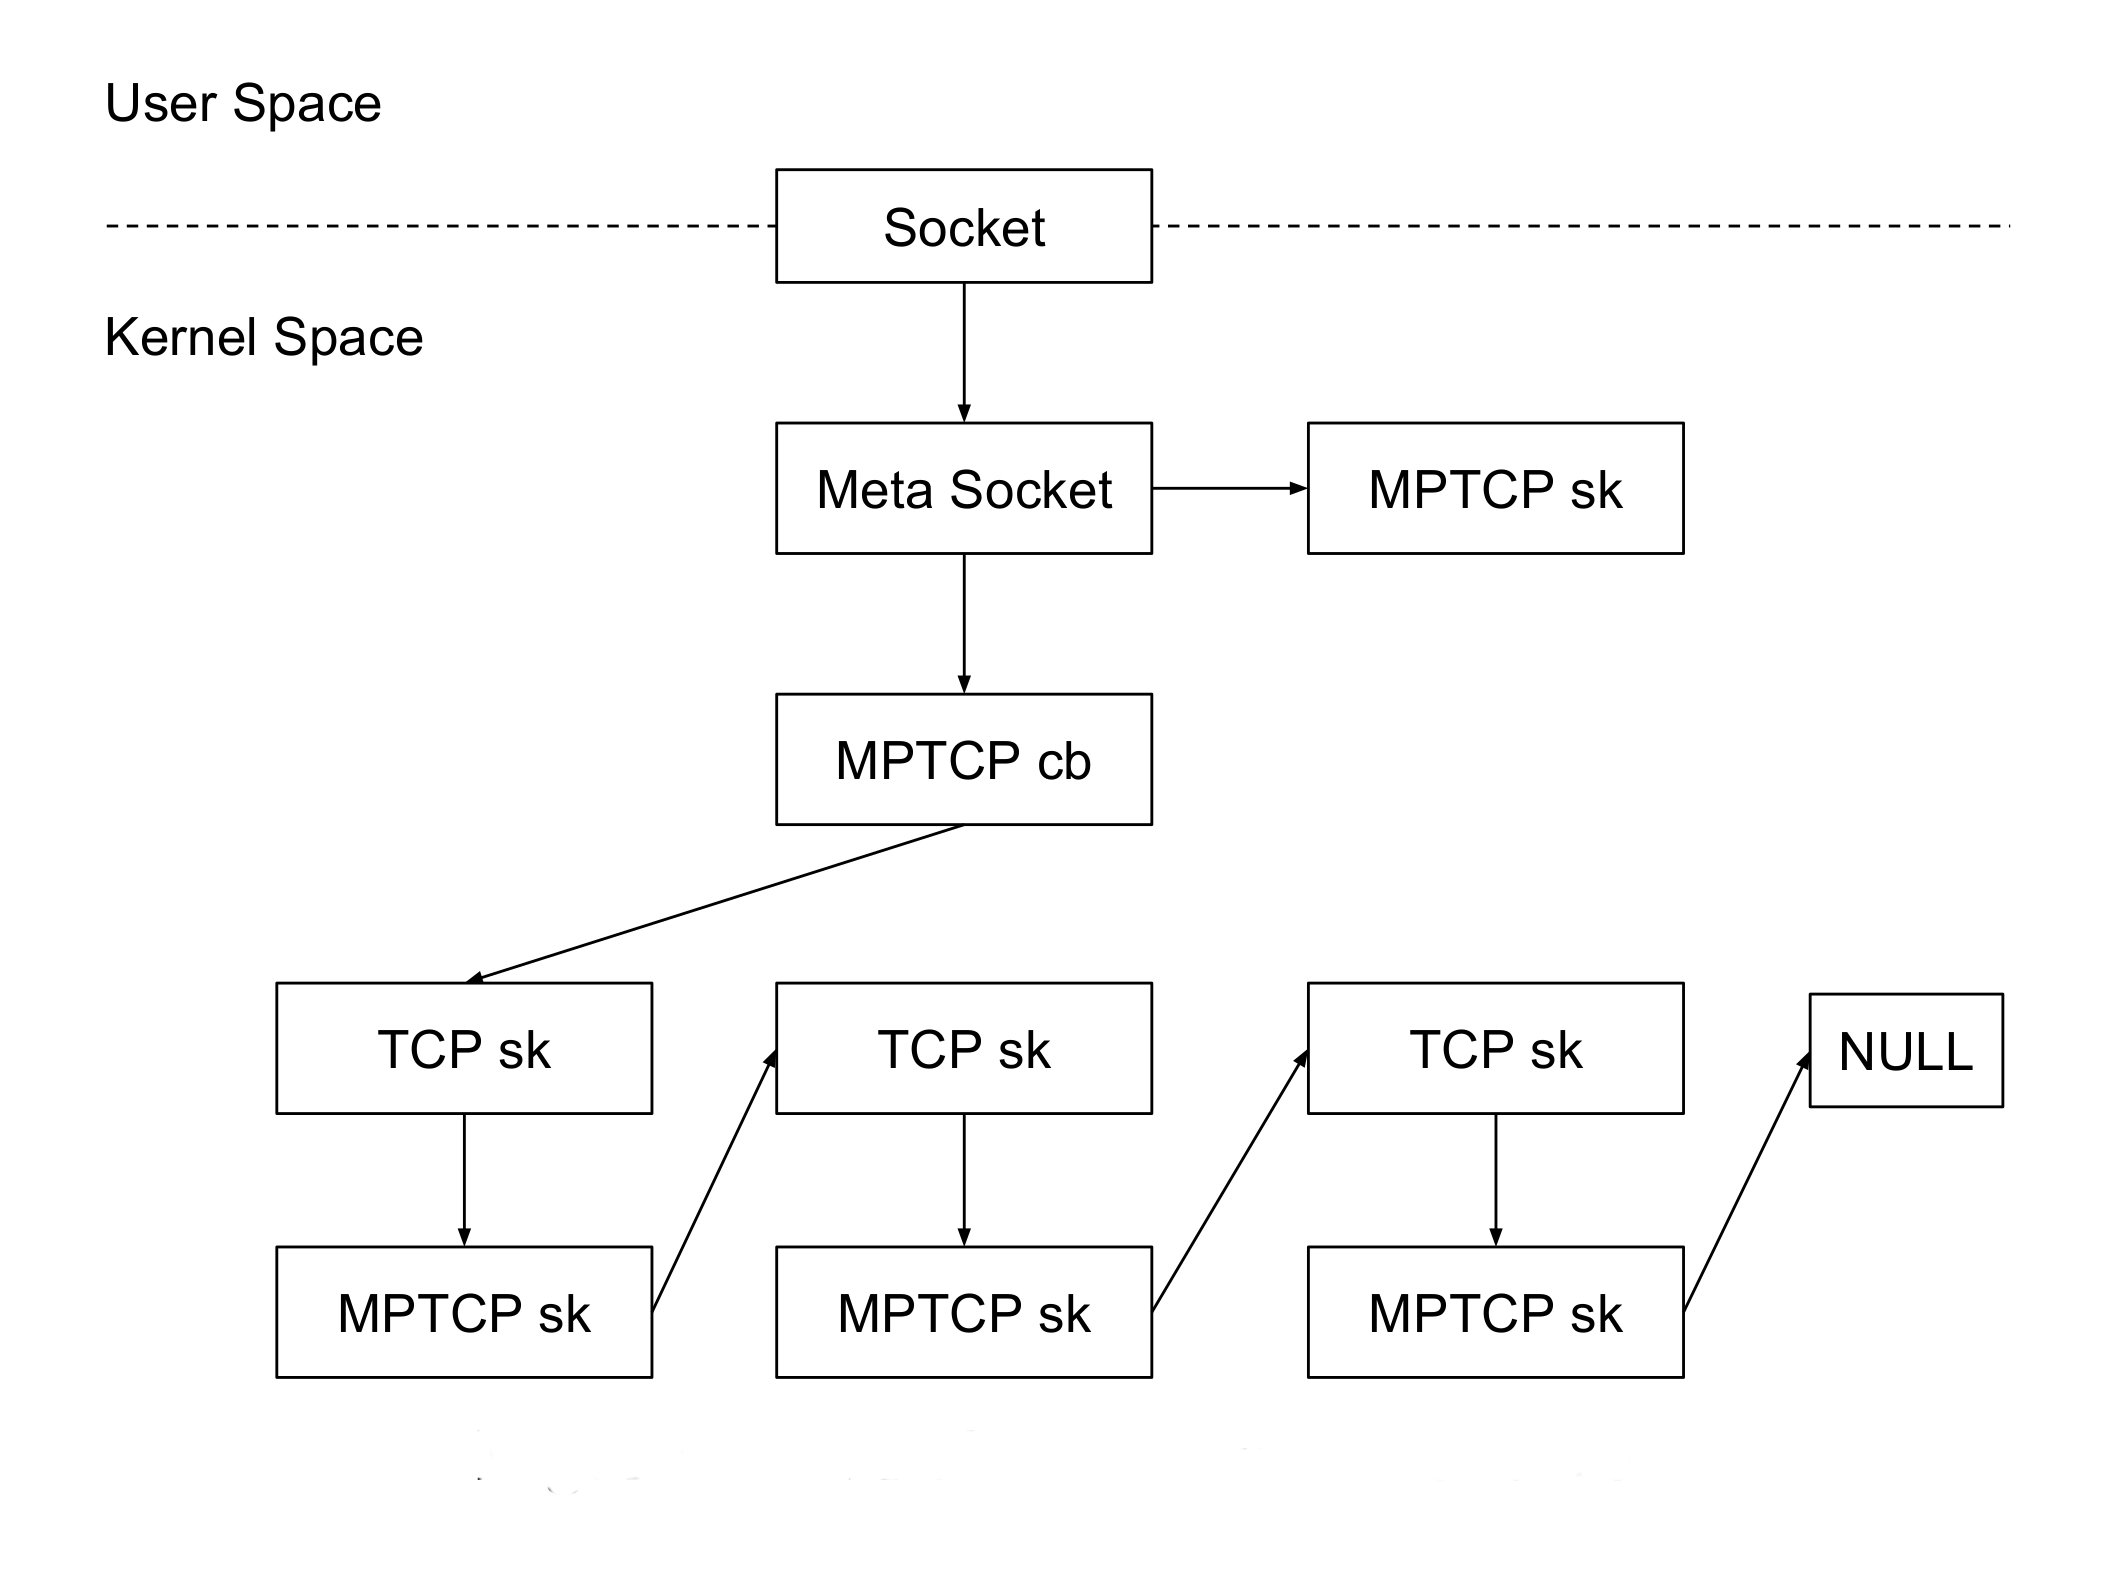
\includegraphics[scale=1.5]{pictures/mptcp_socket_structure.jpg}
				\caption[]{MPTCP socket structure}
			\end{center}
			\end{figure}

			From the application's point of view, no other socket other than the \textbf{Meta Socket} is visible. Underneath the \textbf{Meta Socket} lie several subsockets, each representing a sub flow. The structure \textbf{mptcp\_cb} points towards the head of the subflow list. The structure \textbf{mptcp\_sk} hence points indirectly towards the next subflow.
			Till now there is no way for the application to know what hides beyond the \textbf{Meta Socket}. This is where the socket options come into play. The enhanced socket API lists the following socket options for the user \cite{api}:

			\begin{table}[h]
				
				

				\begin{tabular}{|l|c|c|r|}
					\hline
					Name & Input & Output & Description \\
					\hline
					\hline
					MPTCP\_GET\_SUB\_IDS & - & subflow list & Get the current list of \\&&&subflows viewed by the kernel \\
					\hline
					MPTCP\_GET\_SUB\_TUPLE & id & sub tuple & Get the ip and ports used by \\&&&the subflow identified by id \\
					\hline
					MPTCP\_OPEN\_SUB\_TUPLE & tuple & - & Request a new subflow with \\&&&pair of ip and ports \\
					\hline
					MPTCP\_CLOSE\_SUB\_ID & id & - & Close the subflow identified \\&&&by id \\
					\hline
					MPTCP\_SUB\_GETSOCKOPT & id, sock opt & sock ret & Redirects the getsockopt given \\&&&in input to the subflow \\&&&identified by id and return the \\&&&value returned by the operation \\
					\hline
					MPTCP\_SUB\_SETSOCKOPT & id, sock opt & - & Redirects the setsockopt given \\&&&in input to the subflow \\&&&identified by id \\
					\hline

				\end{tabular}
				\caption{Implemented MPTCP socket options}
			\end{table}

			\raggedright{The following example shows how we may use the socket option \textbf{MPTCP\_OPEN\_SUB\_TUPLE} and \textbf{getsockopt()}to open a sub flow \cite{api}:}

			First we introduce the \textbf{mptcp\_sub\_tuple} structure which represents the subflow :
			\begin{lstlisting}
			struct mptcp_sub_tuple {
				_u8 id;			// this is an output signifying the ``id'' of the subflow
				_u8 prio;		// this field determines if the sub flow is backup or not
				_u8 addrs[0];	// pair array of size two depicting (source, destination)
			}
			\end{lstlisting}
			Now we use this structure to open a sub flow as follows :
			\begin{lstlisting}
   			unsigned int optlen;
   			struct mptcp_sub_tuple *sub_tuple;
   			struct sockaddr_in *addr;
   			optlen = 42;

   			int error;

   			optlen = sizeof(struct mptcp_sub_tuple) + 2 * sizeof(struct sockaddr_in);
   			sub_tuple = malloc(optlen);

   			sub_tuple->id = 0;
   			sub_tuple->prio = 0;

   			addr = (struct sockaddr_in*) &sub_tuple->addrs[0];

   			// source address
   			addr->sin_family = AF_INET; // address family IPv4
   			addr->sin_port = htons(12345); // source port
   			inet_pton(AF_INET, "10.0.0.1", &addr->sin_addr); // source IP

   			addr++;

   			// destination address
   			addr->sin_family = AF_INET; // address family IPv4
   			addr->sin_port = htons(1234); // destination port
   			inet_pton(AF_INET, "10.1.0.1", &addr->sin_addr); // destination IP

   			error = getsockopt(sockfd, IPPROTO_TCP, MPTCP_OPEN_SUB_TUPLE,
                    sub_tuple, &optlen); // establishment of sub flow using getsockopt()
			\end{lstlisting}

		The result is a flow from the pair \textbf{(10.0.0.1: 12345)} to the pair \textbf{(10.1.0.1: 1234)}.

	
	\section{Netcat with MPTCP (netcat-mptcp) :}
		\label{sec:netcat-mptcp}
		In order to have a concrete testbed for the enhanced socket API, we have thought of a usecase involving \textbf{Netcat}. \textbf{Netcat} or \textbf{nc} is a featured networking utility which reads and writes data across network connections, using the TCP/IP protocol \cite{nc}. It will serve as our application that will establish multiple subflows.

		\subsection{Setup and structure}
			\label{subsec:setup}
			Usually with \textbf{Netcat}, there is only one flow between a client and a server. Our objective is to have multiple interfaces on the client side which will connect to the same or multiple interfaces on the server side. For simplicity we have envisaged a scenario where the client has three interfaces (viz. default, wifi and cellular) and the server has three. However for demonstration purposes we need to connect to only one of them. Our goal after the modifications is to use either the Cellular or Wifi or both interfaces, the interface type and address being defined in a configuration file accessible by the client. The way the client connects to the server is changed. In fact, with our modifications in the source code, we are able to pass three additional arguments in the netcat command :

			\begin{enumerate}
				\item \textbf{-a} : Find all the remaining interfaces on the client side and establish sub flows to the server.
				\item \textbf{-W} : Read the configuration file, extract the IP corresponding to the wifi interface and establish a sub flow using this interface to the server.
				\item \textbf{-C} : Read the configuration file, extract the IP corresponding to the cellular interface and establish a sub flow using this interface to the server.
			\end{enumerate}

			For our purpose, we need the kernel not to do anything \emph{suo moto}. Hence the \textbf{path\_manager} used is the \textbf{``default'' path\_manager}. What happens after our modifications is that the client connects to the server via the default interface as usual. Then according to the option passed in the \textbf{Netcat} command, it either opens a subflow on the default interface or in addition on a subset of all available interfaces. This is done using the function \emph{getsockopt()} in the source code just after the TCP \emph{connect()} system call. \\
			The following diagram depicts the setup along with the addresses :
			\begin{figure}[h]
				\begin{center}
					\label{fig:topology}
					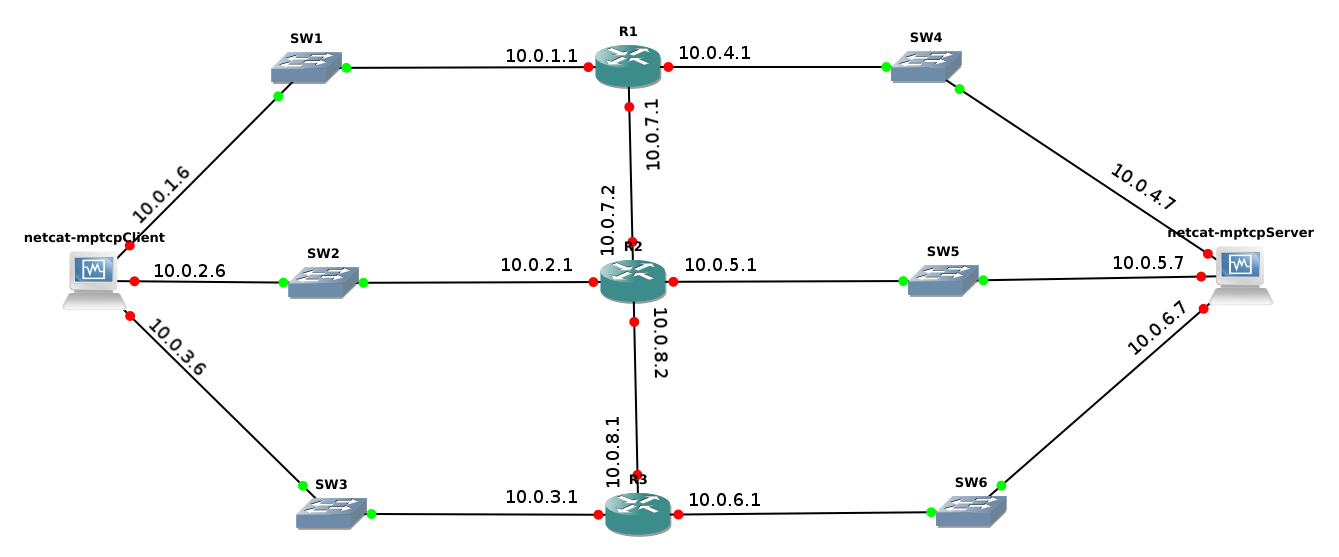
\includegraphics[scale=0.45]{pictures/topologie.jpg}
					\caption[]{Testbed topology for netcat-mptcp}
				\end{center}
			\end{figure}

			Here is an example of the \textbf{Netcat} command : \\
			On the server side, it listens on it's default interface \textbf{10.0.4.7} on port \textbf{64000} with the help of the following command : \\

			\textbf{nc -l -p 64000} \\

			On the client side, we use our own \textbf{Netcat} executable to establish a flow / multiple flows as follows :

			
			\begin{tabbing}
			-a : ~~~~~~~~\=\textbf{./netcat-mptcp/src/netcat -a 10.0.4.7 64000} \\
			-W : \> \textbf{./netcat-mptcp/src/netcat -W 10.0.4.7 64000} \\
			-C : \> \textbf{./netcat-mptcp/src/netcat -C 10.0.4.7 64000}
			\end{tabbing}


		\subsection{Configure Addresses and Routing}
			\label{subsec:addressandroute}
			For the testbed, we have set up the above topology on \textbf{GNS3} using the Cisco Router \textbf{c3745} and the virtual machine enabled with the enhanced Multipath TCP API.

			\subsection{Client and Server}
			\label{subsec:clientandserver}
			The following command example assigns the address \textbf{10.0.1.6} to the interface \textbf{eth0} : \\
			\textbf{\emph{Client side :}} \\
			\begin{lstlisting}
			ip addr add 10.0.1.6/24 dev eth0
			\end{lstlisting}
			Appendix \hyperref[subsec:clientaddress]{10.1} and \hyperref[subsec:serveraddress]{10.2} illustrate the scripts that are run to assign addresses on the client side and the server side.

			With multiple addresses defined on several interfaces, we would also like to tell the kernel to use specific interfaces and gateways and not the default ones acccording to the source addresses. This has been achieved by configuring one routing table per outgoing interface, each routing table being identified by a number. The route selection process then happens in two phases : First the kernel does a lookup in the policy table (that we need to configure with \textbf{\emph{ip rules}}). The policies in our case, will be that for so and so source prefix, go to so and so routing table (the routing table indicated by a number). The corresponding routing table is examined to select the gateway based on the destination addresses \cite{routing}.

			Appendix \hyperref[subsec:clientroute]{10.3} and \hyperref[subsec:serverroute]{10.5} illustrate the scripts that are run to manually configure the routing policies on the client side and the server side.

			Appendix \hyperref[subsec:clientrouteout]{10.4} and \hyperref[subsec:serverrouteout]{10.6} illustrate the outputs for the different commands for showing the routing policies.

			\subsection{Routers}
			\label{subsec:router}
			In figure \hyperref[fig:topology]{2} the three routes need to be configured to properly deliver packets to the correct destination.
			We have connected to the routers via telnet to configure them.

			Appendix \hyperref[subsec:routerconf1]{10.7}, \hyperref[subsec:routerconf2]{10.9} and \hyperref[subsec:routerconf3]{10.11} illustrate the commands that must be given to the routers \textbf{R1, R2} and \textbf{R3} respectively.


			Appendix \hyperref[subsec:routerconfout1]{10.8}, \hyperref[subsec:routerconfout2]{10.10} and \hyperref[subsec:routerconfout3]{10.12} illustrate the outputs for the \textbf{sh ip route} command.

		\subsection{Code simplification, addition and function calls at the correct place}
			\label{subsec:codesimplify}
			The above code involving opening a sub flow may appear complex. During our participation at the \textbf{IETF'97 Hackathon} at \textbf{École Polytechnique de Louvain} \cite[hackathon]{ucl}, one of my fellow participants had simplified the usage of the \textbf{getsockopt()} function by deploying simpler function calls. Our aim was to find in the source code of \textbf{Netcat} where the \textbf{connect()} system call was being made. Once the the exact place found, we were to simply use the subflow opening code in the simplified form and establish the desired subflows. We have added three different scenarios for the establishment of subflows as described in the section \hyperref[subsec:setup]{Setup and structure}. We have three different options while the \textbf{Netcat} connection : \textbf{``-a''} for opening subflows on all remaining interfaces, \textbf{``-C''} for opening a subflow on the Cellular interface and \textbf{``-W''} for opening a subflow on the Wifi interface.

			Besides the classes \textbf{\emph{makeaddr.c, subinfo.c, submanip.c and suboption.c}} and the header files \textbf{\emph{makeaddr.h, subinfo.h, submanip.h and suboption.h}} which are required simplify the opening of subflows and which are available at the \textbf{src} folder of the github repository : \cite[https://github.com/lawrenceFR/netcat-mptcp]{github}, the following addition of code was also necessary for the proper functioning of \textbf{\emph{netcat-mptcp}} :
			\begin{enumerate}
				\item In \textbf{\emph{netcat-mptcp/src/Makefile.am}} line \textbf{28 - 39} : Appendix \hyperref[subsec:Makefile.am]{Makefile.am} \\
				Required to include the added \textbf{.c} files during \textbf{make}.

				\item In \textbf{\emph{netcat-mptcp/src/Makefile.in}} line \textbf{153 - 164} and \textbf{183 - 186} : Appendix \hyperref[subsec:Makefile.in]{Makefile.in} \\
				Required to include the added \textbf{.c} files during \textbf{make}.

				\item In \textbf{\emph{netcat-mptcp/src/netcat.h}} line \textbf{203 - 205} : Appendix \hyperref[subsec:netcat.h]{netcat.h} \\
				Here we declare the three options as \textbf{extern} variables.

				\item In \textbf{\emph{netcat-mptcp/src/netcat.c}} line \textbf{58 - 60}, \textbf{192}, \textbf{194}, \textbf{222}, \textbf{227}, \textbf{233 - 235}, \textbf{239 - 241}, \textbf{357 - 359} : Appendix \hyperref[subsec:netcat.c]{netcat.c} \\
				Here we add the three cases corresponding to the three different options (\textbf{switch} variable).

				\item In \textbf{\emph{netcat-mptcp/src/core.h}} line \textbf{1 - 37} : Appendix \hyperref[subsec:core.h]{core.h} \\
				Here we declare the variables and methods that we have defined and used in \textbf{core.c} in order to bring about the modifications.

				\item In \textbf{\emph{netcat-mptcp/src/core.c}} line \textbf{394 - 405} and \textbf{535 - 688} : Appendix \hyperref[subsec:core.c]{core.c} \\
				Here we define the functions that bring in the actual modifications in the functioning of \textbf{Netcat}.
			\end{enumerate}

			Finally, a file \textbf{config.conf} is placed in \textbf{netcat-mptcp/src} so as to indicate the addresses of the available interfaces. The format of the config file is shown in Appendix \hyperref[subsec:config.conf]{config.conf}.
			
	\clearpage
	\section{Results, Statistics and Utility}
		\label{sec:res}
		This section analyses packet captures (captured with the help of \textbf{Wireshark} with a topology simulation on \textbf{GNS3}) to verify if the manipulation of \textbf{Netcat} was successful. It depicts the establishment of the different sub flows along with the details of the \textbf{TCP options} to prove that the \textbf{MP\_CAPABLE} option is actually passed. It also gives an idea of the distribution of packets sent from the three interfaces available on the client's side, keeping in mind that the \textbf{path\_manager} used is \textbf{``default''} (i.e. the kernel will not establish supplementary sub flows on its own).
		\subsection{Results}
			\label{subsec:result}
			Figure \hyperref[fig:synack]{3} is a screenshot of a packet capture showing that the kernel successfully establishes the second and third sub flows when we use the option \textbf{-a} as explained previously. First, the see the \textbf{3 way handshake} from the client address \textbf{10.0.1.6} to the server address \textbf{10.0.4.7}. Next due our the manipulation in the \textbf{Netcat} source code we have the two other \textbf{3 way hanshakes} from the client addresses \textbf{10.0.2.6} and \textbf{10.0.3.6}. This is in accordance with the function of the option \textbf{-a} in the \textbf{Netcat} command defined by us (i.e. establish supplementary sub flows on all the remaining available interfaces of the client).
			\begin{figure}[h]
				\begin{center}
					\label{fig:synack}
					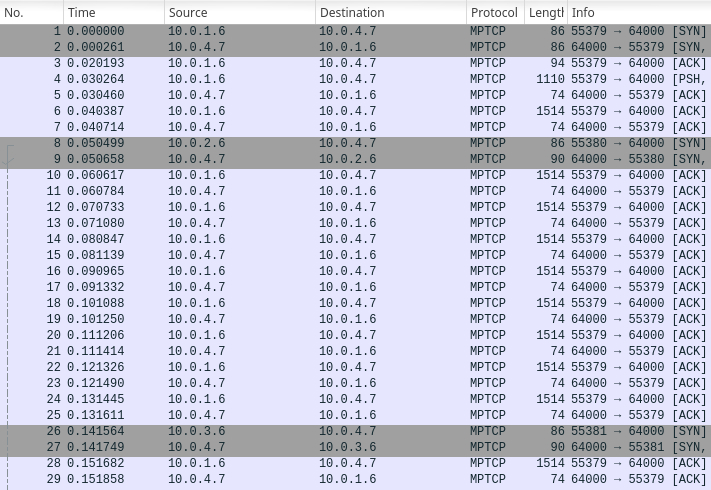
\includegraphics[scale=0.5]{pictures/synack.jpg}
					\caption[]{Subflow establishment}
				\end{center}
			\end{figure}

			The following figures give the details of the \textbf{TCP options} for the first sub flow established. We see the \textbf{Multipath Capable} option that is passed :

			
			\begin{figure}[h!]
			\centering
			\label{fig:firstsubflow}
			\begin{subfigure}{.5\textwidth}
			  \centering
			  \label{fig:firstflow}
			  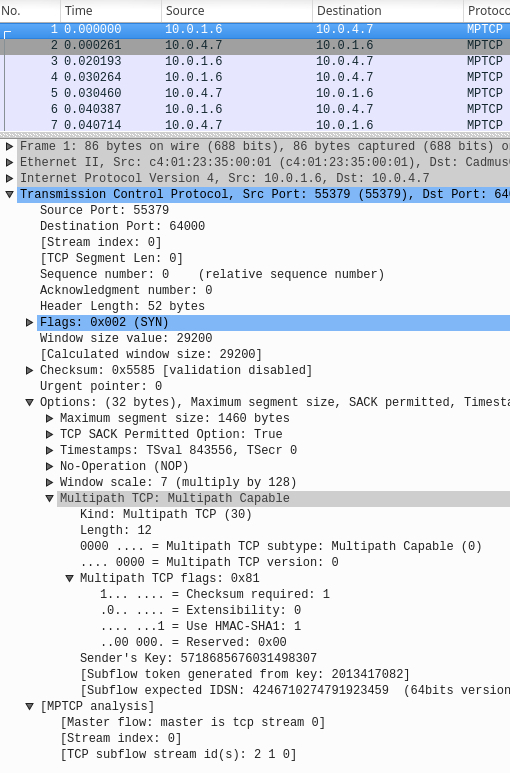
\includegraphics[width=0.8\linewidth]{pictures/firstflow.jpg}
			  \caption{First subflow SYN}
			\end{subfigure}%
			\begin{subfigure}{.5\textwidth}
			  \centering
			  \label{fig:firstflowresponse}
			  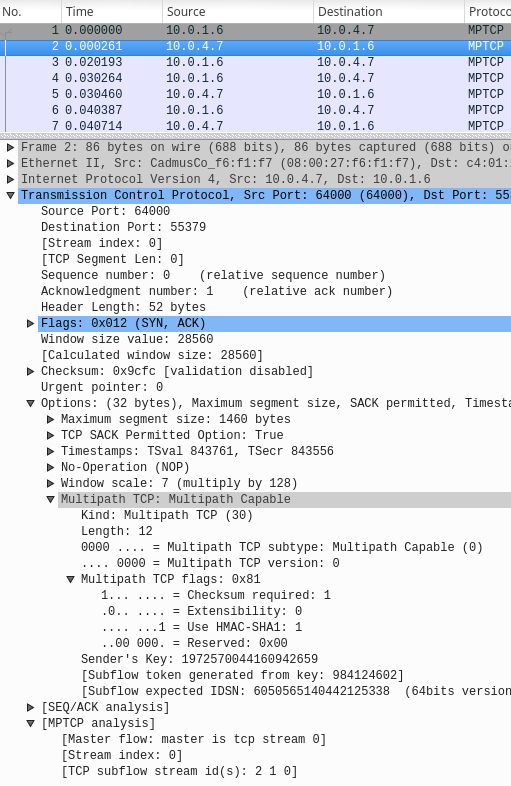
\includegraphics[width=0.8\linewidth]{pictures/firstflowresponse.jpg}
			  \caption{First subflow SYN + ACK}
			\end{subfigure}
			\caption{First subflow details}
			\end{figure}

			\begin{figure}[h!]
			\centering
			\label{fig:firstflowack}
			\begin{subfigure}{.5\textwidth}
			  \centering
			  \label{fig:firstflow}
			  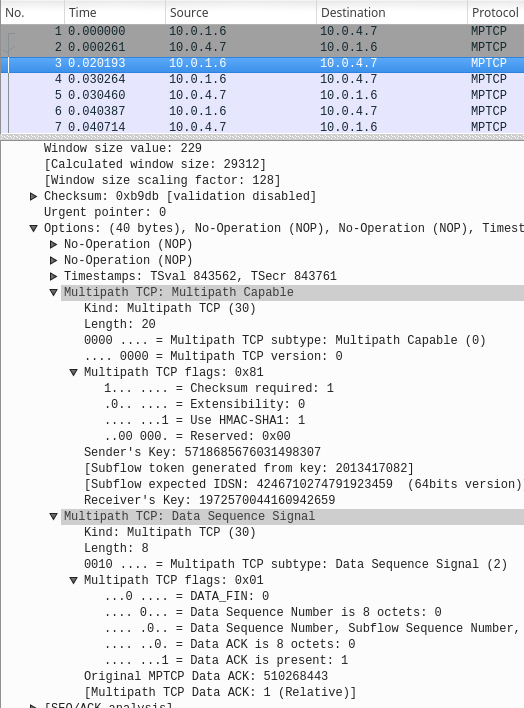
\includegraphics[width=0.8\linewidth]{pictures/firstflowack.jpg}
			\end{subfigure}%
			\begin{subfigure}{.5\textwidth}
			  The \textbf{3 way handshake} illustrates the key exchange procedure. We see that the \textbf{Multipath Capable} option contains the sender and receiver tokens. This ensures the security aspect of \textbf{MPTCP}. The \textbf{SYN} contains the client's key. The \textbf{SYN + ACK} contains the server's key. Finally the client replies with an \textbf{ACK} containing both the keys. \\
			  \\
			  In the following figures the second and third subflows contain the \textbf{TCP option Join Connection} proving the usage of \textbf{MP\_JOIN}.
			\end{subfigure}
			\caption{First subflow ACK}
			\end{figure}

			

			
			\begin{figure}[h!]
			\centering
			\label{fig:secondsubflow}
			\begin{subfigure}{.5\textwidth}
			  \centering
			  \label{fig:secondflow}
			  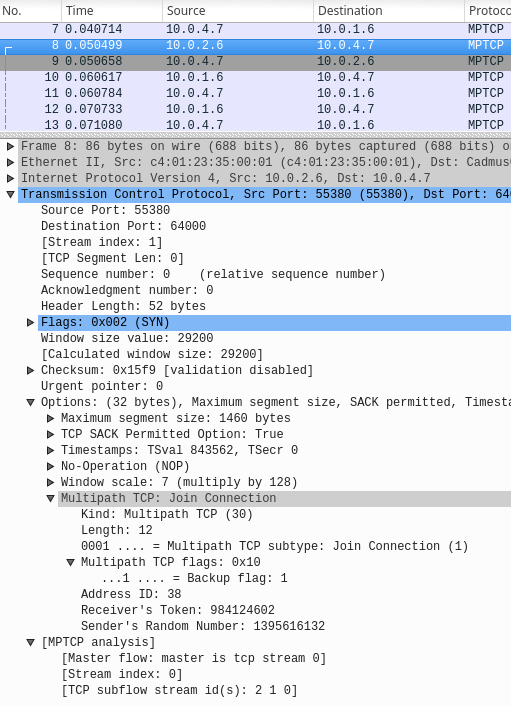
\includegraphics[width=.8\linewidth]{pictures/secondflow.jpg}
			  \caption{Second subflow SYN}
			\end{subfigure}%
			\begin{subfigure}{.5\textwidth}
			  \centering
			  \label{fig:secondflowresponse}
			  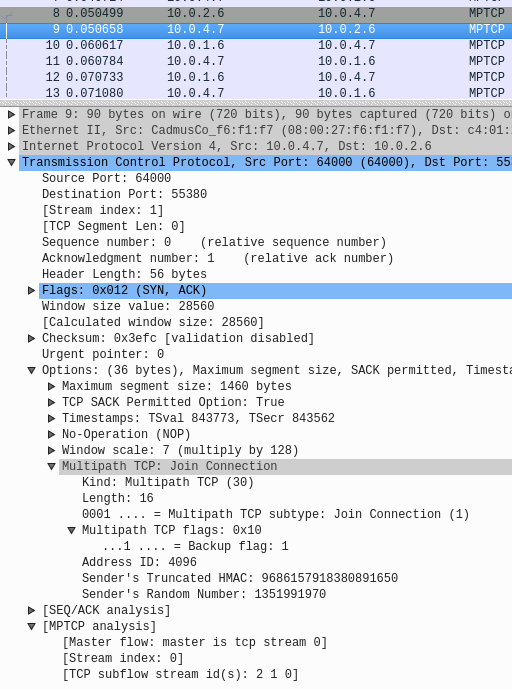
\includegraphics[width=.8\linewidth]{pictures/secondflowresponse.jpg}
			  \caption{Second subflow SYN + ACK}
			\end{subfigure}
			\caption{Second subflow details}
			\end{figure}

			
			\begin{figure}[h!]
			\centering
			\label{fig:thirdsubflow}
			\begin{subfigure}{.5\textwidth}
			  \centering
			  \label{fig:secondflow}
			  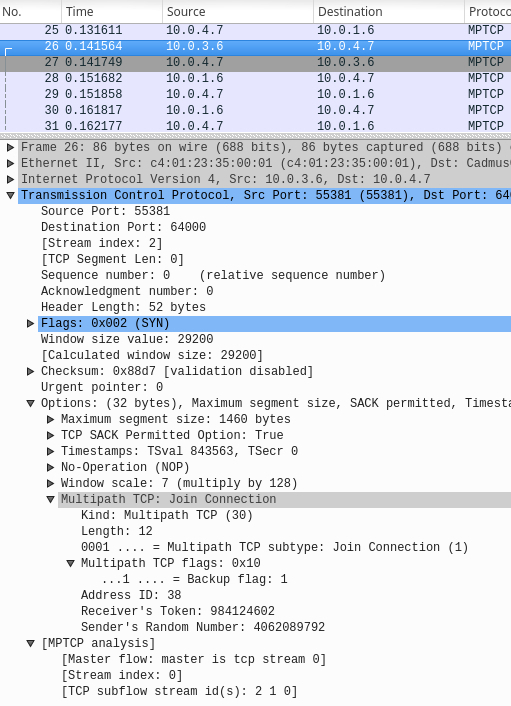
\includegraphics[width=.8\linewidth]{pictures/thirdflow.jpg}
			  \caption{Third subflow SYN}
			\end{subfigure}%
			\begin{subfigure}{.5\textwidth}
			  \centering
			  \label{fig:thirdflowresponse}
			  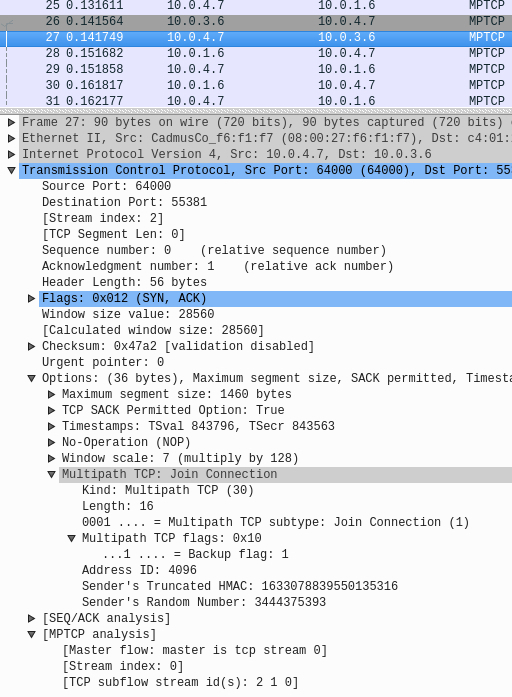
\includegraphics[width=.8\linewidth]{pictures/thirdflowresponse.jpg}
			  \caption{Third subflow SYN + ACK}
			\end{subfigure}
			\caption{Third subflow details}
			\end{figure}


	\clearpage
		\subsection{Statistics}
			\label{subsec:statistics}
			This section mentions a few statistics regarding the performance of \textbf{MPTCP} once the supplementary subflows are established.\\
			\subsubsection{IPv4/All Addresses packet distribution}
			\label{subsubsec:packetdistribution}
			Our first look is at the \textbf{IPv4/All Addresses} packet distribution which indicates the percentage contribution of each interface in the exchange of data. We have tried to send a fixed amount of random data (10MB) at bulks of 1MB for 10 counts. Command on the client side :\\
			\textbf{dd if=/dev/zero bs=1M count=10 | ./netcat-mptcp/src/netcat -a 10.0.4.7 64000}

			\begin{table}[h]
				
				
				\centering
				\begin{tabular}{|c|c|c|c|c|c|}
					\hline
					IP & Count & Rate(ms) & Percent & Burst rate & Burst start \\
					\hline
					\hline
					10.0.4.7 & 14076 & 0.1870 & 100.00\% & 0.2200 & 64.072 \\
					\hline
					10.0.3.6 & 3331 & 0.0442 & 23.66\% & 0.2000 & 0.890 \\
					\hline
					10.0.2.6 & 5021 & 0.0667 & 35,67\% & 0.2000 & 0.516 \\
					\hline
					10.0.1.6 & 5724 & 0.0760 & 40.66\% & 0.2000 & 0.223 \\
					\hline
				\end{tabular}
				\caption{Packet distribution per IPv4 address}
			\end{table}

			The table may seem to show that the distribution of packets is not equal. The interface \textbf{10.0.1.6} seems to send more packets than the others. This is probably due the fact that the packet emission from the second and third interfaces start a little later only after the establishment of the corresponding sub flows. Hence the kernel gets to be aware of the other sub flows later given that the \textbf{path\_manager} used is the \textbf{``default''} one. This is not the case for \textbf{``fullmesh'' path\_manager} as the kernel knows from beforehand that it needs to use all the interfaces available for sending packets. Hence for the \textbf{``fullmesh'' path\_manager} we have an almost equal distribution of packet emission for all the three interfaces.

			\subsubsection{Round Trip Time}
			\label{subsubsec:rtt}
			This section shows the round trip time for the three interfaces. \\
			We see that they are almost the same for the three interfaces (a small exception for the third interface around sequence number 2000000). This shows if the three interfaces are homogeneous in terms of updating their receiving windows and hence the reception and emission of packets. However, when we compare this to the round trip time in the \textbf{``fullmesh'' path\_manager} there is hardly any anomaly in the sense that the round trip time very rarely crosses the \textbf{1800} mark.
			\begin{figure}[h!]
				\begin{center}
					\label{fig:rtt1}
					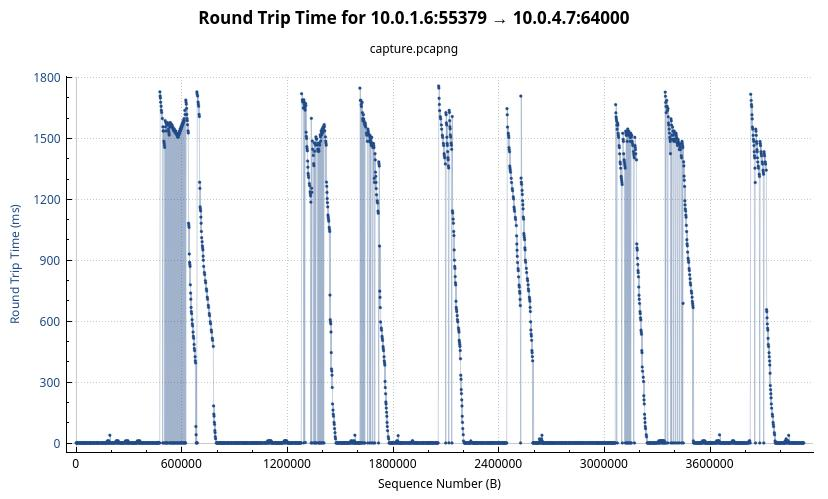
\includegraphics[scale=0.45]{pictures/rtt1.jpeg}
					\caption[]{RTT for 10.0.1.6}
				\end{center}
			\end{figure}
			\begin{figure}[h!]
				\begin{center}
					\label{fig:rtt2}
					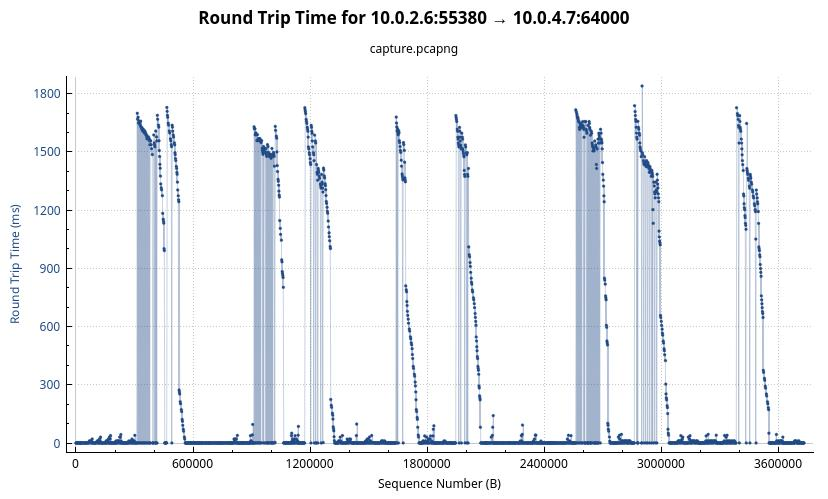
\includegraphics[scale=0.45]{pictures/rtt2.jpeg}
					\caption[]{RTT for 10.0.2.6}
				\end{center}
			\end{figure}
			\begin{figure}[h!]
				\begin{center}
					\label{fig:rtt3}
					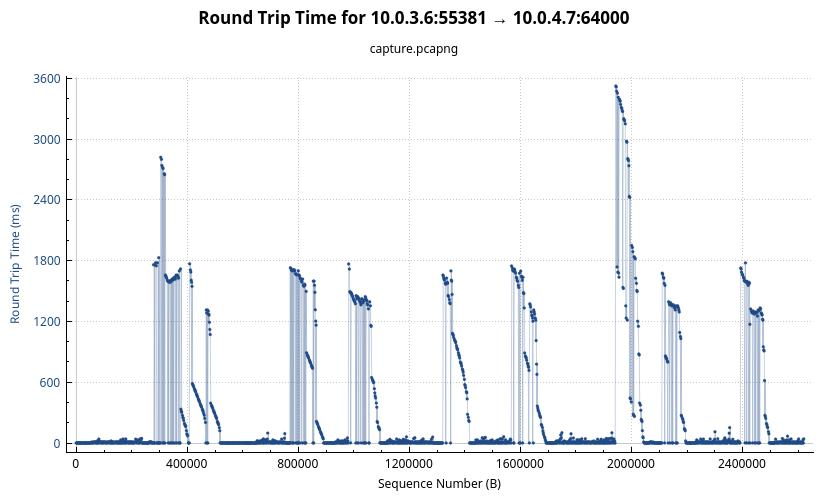
\includegraphics[scale=0.45]{pictures/rtt3.jpeg}
					\caption[]{RTT for 10.0.3.6}
				\end{center}
			\end{figure}

			\clearpage
			\subsubsection{Cumulative Bytes}
			\label{subsubsec:cumbytes}
			This section illustrates the comparison of the number of bytes sent in due course of time for the three interfaces of the client. On the Y-axis we have the cumulative number of bytes. This figure shows that the interfaces \textbf{10.0.1.6} and \textbf{10.0.2.6} run almost parallel to one another, which means that their throughput is similar. The offset is attributed to the fact that the second interface starts to send packets later. For the third interface \textbf{10.0.3.6} the throughput seems to be less compared to the other two.
			\begin{figure}[h!]
				\centering
					\label{fig:cumbytes}
					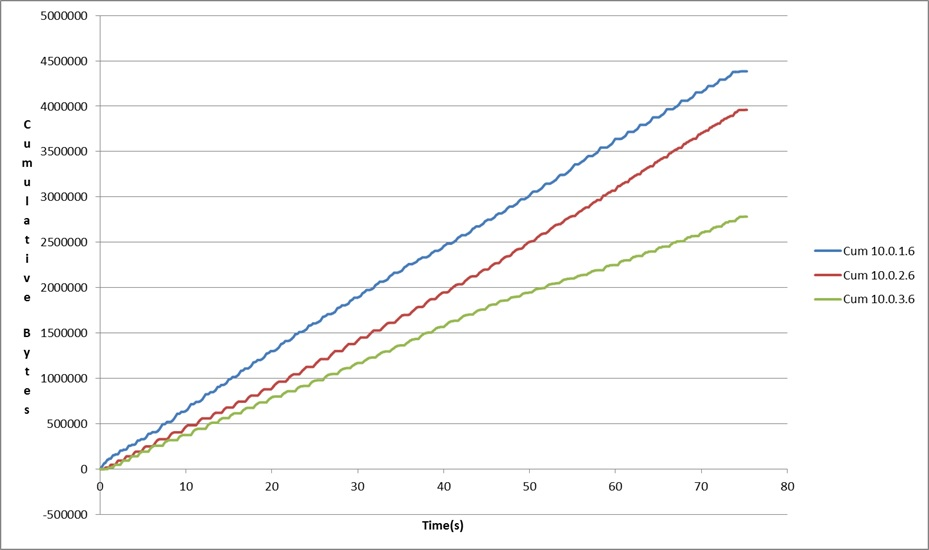
\includegraphics[scale=0.5]{pictures/cumbytes.jpg}
					\caption[]{Cumulative of bytes sent for the three interfaces}
			\end{figure}

			\subsubsection{Data transfer and flow establishment statistics}
			\label{subsubsec:datatransferandflowestablish}
			In this section we talk about the latency, the rate of data transfer and the interval lapse among the sub flows for the two cases. The first case is where we use the \textbf{``fullmesh'' path\_manager} and establish a \textbf{Netcat} connection without any of the three defined command options. The second case is where we use the \textbf{``default'' path\_manager} and the defined \textbf{Netcat} command option \textbf{``-a''} to open sub flows on the remaining available interfaces. \\

			To compare the two cases we caculate the mean and standard deviation for the different measures. \\

			The mean is given by the formula :
			$$\mu = \frac{1}{n}\sum_{i=1}^{n}x_i$$
			The standard deviation is given by the formula :
			$$\sigma = \sqrt{\frac{1}{n}\sum_{i=1}^{n}(x_i - \mu)^2}$$
			In the experiment, we sent 10MB of random data at bulks of 1MB for 10 counts from the client to the server using the command : \\
			\textbf{dd if=/dev/zero bs=1M count=10 | ./netcat-mptcp/src/netcat -a 10.0.4.7 64000} \\
			The experiment was repeated 10 times.

			\paragraph{Data Transfer : }
			\label{subsubsubsec:datatransfer}
			After sending 10MB of data it was seen that in the two cases, the rate of data transfer and hence the duration was drastically different. The observations were as follows :
			\begin{table}[h!]
				
				
				\centering
				\begin{tabular}{|c|c|c|c|c|c|}
					\hline
					Obs & \multicolumn{2}{|c|}{Fullmesh} &  & \multicolumn{2}{|c|}{Default} \\
					\hline
					\hline
					& Rate(kB/s) & Time(s) &  & Rate(kB/s) & Time(s) \\
					\hline
					\hline
					1 & 515 & 20.3492 &  & 153 & 68.4308 \\
					\hline
					2 & 516 & 20.3332 &  & 147 & 71.4054 \\
					\hline
					3 & 549 & 19.105 &  & 151 & 69.5162 \\
					\hline
					4 & 551 & 19.0169 &  & 152 & 68.7636 \\
					\hline
					5 & 463 & 22.6526 &  & 149 & 70.567 \\
					\hline
					6 & 521 & 20.1181 &  & 151 & 69.6091 \\
					\hline
					7 & 502 & 20.8867 &  & 150 & 69.7403 \\
					\hline
					8 & 446 & 23.4884 &  & 156 & 67.2153 \\
					\hline
					9 & 507 & 20.7018 &  & 148 & 70.8937 \\
					\hline
					10 & 515 & 20.3454 &  & 157 & 66.5856 \\
					\hline
				\end{tabular}
				\caption{Data transfer rate and time taken to send 10MB from client to server}
			\end{table} \\
			We define :
			$$\mu_{fm}^{rate} := mean\ of\ data\ transfer\ rate\ for\ fullmesh\ configuration$$ 
			$$\mu_{df}^{rate} := mean\ of\ data\ transfer\ rate\ for\ default\ configuration$$
			$$\sigma_{fm}^{rate} := standard deviation\ of\ data\ transfer\ rate\ for\ fullmesh\ configuration$$
			$$\sigma_{df}^{rate} := standard deviation\ of\ data\ transfer\ rate\ for\ default\ configuration$$

			From our observations we have :
			$\mu_{fm}^{rate} = 508.5\ kB/s$ and $\mu_{df}^{rate} = 151.4\ kB/s$
			Hence we observe that the data transfer rate is reduced when we initiate subflows from the application level. In case of \textbf{``fullmesh''}, it is the kernel that initiates the subflows.
			Next if we compare the standard deviations in the two cases. While $\sigma_{fm}^{rate} = 31.2482\ kB/s$, $\sigma_{df}^{rate} = 3.07246\ kB/s$. This shows that in case of \textbf{``fullmesh''}, the fluctuation of bandwidth is higher. The same conclusions may be drawn for the total time taken to transfer 10MB ranfom data in the two cases.

			\clearpage
			\paragraph{Flow establishment statistics :}
			\label{subsubsubsec:flowestablish}
			Here we compare the time intervals among the first, second and third subflow establishments. The observations were as follows :
			\begin{table}[h!]
				
				
				\centering
				\begin{tabular}{|c|c|c|c|c|c|c|c|}
					\hline
					Obs & \multicolumn{3}{|c|}{Fullmesh} &  & \multicolumn{3}{|c|}{Default} \\
					\hline
					\hline
					& flow1 - flow2 & flow2 - flow3 & flow1 - flow3 & & flow1 - flow2 & flow2 - flow3 & flow1 - flow3 \\
					\hline
					\hline
					1 & 0.172115 & 0.030324 & 0.202439 & & 0.030288 & 0.111036 & 0.141324 \\
					\hline
					2 & 0.171439 & 0.030272 & 0.201711 & & 0.030233 & 0.111062 & 0.141295 \\
					\hline
					3 & 0.171637 & 0.030321 & 0.201958 & & 0.131091 & 0.010066 & 0.141157 \\
					\hline
					4 & 0.171403 & 0.030351 & 0.201754 & & 0.131221 & 0.010084 & 0.141305 \\
					\hline
					5 & 0.171689 & 0.030322 & 0.202011 & & 0.130997 & 0.010079 & 0.141076 \\
					\hline
					6 & 0.171472 & 0.030259 & 0.201731 & & 0.131214 & 0.010097 & 0.141311 \\
					\hline
					7 & 0.171598 & 0.030268 & 0.201866 & & 0.030258 & 0.11108 & 0.141338 \\
					\hline
					8 & 0.171551 & 0.030333 & 0.201884 & & 0.130936 & 0.010069 & 0.141005 \\
					\hline
					9 & 0.171399 & 0.010085 & 0.181484 & & 0.030226 & 0.111013 & 0.141239 \\
					\hline
					10 & 0.171555 & 0.030348 & 0.201903 & & 0.131156 & 0.010118 & 0.141274 \\
					\hline
				\end{tabular}
				\caption{Time intervals among the first, second and third flow initiations}
			\end{table} \\
			\iffalse
			We define :
			$$\mu_{fm}^{12} := mean3 of\ time\ interval\ for\ fullmesh\ configuration\ between\ flow1\ and\ flow2$$ 
			$$\mu_{df}^{12} := mean\ of\ time\ interval\ for\ default\ configuration\ between\ flow1\ and\ flow2$$
			$$\mu_{fm}^{23} := mean\ of\ time\ interval\ for\ fullmesh\ configuration\ between\ flow2\ and\ flow3$$ 
			$$\mu_{df}^{23} := mean\ of\ time\ interval\ for\ default\ configuration\ between\ flow2\ and\ flow3$$
			$$\mu_{fm}^{31} := mean\ of\ time\ interval\ for\ fullmesh\ configuration\ between\ flow3\ and\ flow1$$ 
			$$\mu_{df}^{31} := mean\ of\ time\ interval\ for\ default\ configuration\ between\ flow3\ and\ flow1$$
			$$\sigma_{fm}^{12} := standard\ deviation\ of\ time\ interval\ for\ fullmesh\ configuration\ between\ flow1\ and\ flow2$$
			$$\sigma_{df}^{12} := standard\ deviation\ of\ time\ interval\ for\ default\ configuration\ between\ flow1\ and\ flow2$$
			$$\sigma_{fm}^{23} := standard\ deviation\ of\ time\ interval\ for\ fullmesh\ configuration\ between\ flow2\ and\ flow3$$
			$$\sigma_{df}^{23} := standard\ deviation\ of\ time\ interval\ for\ default\ configuration\ between\ flow2\ and\ flow3$$
			$$\sigma_{fm}^{31} := standard\ deviation\ of\ time\ interval\ for\ fullmesh\ configuration\ between\ flow3\ and\ flow1$$
			$$\sigma_{df}^{31} := standard\ deviation\ of\ time\ interval\ for\ default\ configuration\ between\ flow3\ and\ flow1$$
			\fi
			We define for $i,j \in \{1, 2, 3\}$:
			$$\mu_{fm}^{ij} := mean\ of\ time\ interval\ for\ fullmesh\ configuration\ between\ flowi\ and\ flowj$$ 
			$$\mu_{df}^{ij} := mean\ of\ time\ interval\ for\ default\ configuration\ between\ flowi\ and\ flowj$$
			$$\sigma_{fm}^{ij} := standard\ deviation\ of\ time\ interval\ for\ fullmesh\ configuration\ between\ flowi\ and\ flowj$$
			$$\sigma_{df}^{ij} := standard\ deviation\ of\ time\ interval\ for\ default\ configuration\ between\ flowi\ and\ flowj$$
			From our observations we have :
			\begin{enumerate}
				\item $\mu_{fm}^{12} = 0.1715858\ s$ and $\mu_{df}^{12} = 0.090762\ s$
				\item $\mu_{fm}^{23} = 0.0282883\ s$ and $\mu_{df}^{23} = 0.0504704\ s$
				\item $\mu_{fm}^{13} = 0.1998741\ s$ and $\mu_{df}^{13} = 0.1412324\ s$ \\
				\item $\sigma_{fm}^{12} = 0.000210408\ s$ and $\sigma_{df}^{12} = 0.052079437\ s$
				\item $\sigma_{fm}^{23} = 0.0063960738\ s$ and $\sigma_{df}^{23} = 0.0521366865\ s$
				\item $\sigma_{fm}^{13} = 0.0064649789\ s$ and $\sigma_{df}^{13} = 0.0001147657\ s$
			\end{enumerate}
			Apart from the differences that we observe in the time intervals of establishment of the sub flows, we also have an idea of the variability of these time intervals from one observation to another.

	\clearpage
	\section{Conclusion}
		\label{sec:conclusion}
	 	This work is the first step towards the usage of the \textbf{Enhanced Socket API for Multipath TCP}. Our objective was to have a first functional prototype for the manipulation of subflows from the \textbf{Application Layer}. With \textbf{Netcat} as our application and the changes in its source code we have been successful in developing a versatile \textbf{netcat-mptcp}. Of course, this is a very preliminary. However the versatality and simplicity of \textbf{netcat-mptcp} will make it easy to bring in any kind of developement of new features and further manipulation.
		 	
		 
	\section{Further developments}
		\label{sec:furtherdevelopment}
		As mentioned in section \hyperref[subsec:statistics]{Statistics}, we have certain underperformances and anomalies that need to be addressed. To list a few of them :

		\begin{enumerate}
			\item \textbf{Equitable packet distribution from the three interfaces of the client} : In \textbf{netcat-mptcp} it is not as fair as in the case of ordinary \textbf{MPTCP} with the \textbf{``fullmesh'' path\_manager}
			\item \textbf{Round Trip Time} : \textbf{Netcat-mptcp} registered some \textbf{RTT}s to be quite large as compared to the \textbf{``fullmesh'' path\_manager} which showed very little variation.
			\item \textbf{Cumulative Bytes for the individual interfaces} : In \textbf{netcat-mptcp} we found that the third interface had a lower throughout. This is contrary to the traditional \textbf{``fullmesh'' path\_manager}.
			\item \textbf{Performance after modifications and further tests} : We observe a declination in the performance in the \textbf{``default'' path\_manager} compared to the \textbf{``fullmesh'' path\_manager}. Our testbed conditions are not optimal to acertain de drop in performance. There are different factors that comme into play such as the allocation of resources while using \textbf{GNS3} etc. Hence we need to retry the observations in a real environment. We may also vary the amount of random data passed (1MB, 10MB, 100MB etc.) to see how the graphs evolve.
		\end{enumerate}

		There might be other glitches which may come up in the course of further developement of \textbf{netcat-mptcp}. However, the current version is functional and attains the objective of manipulation of \textbf{MPTCP} subflows from the \textbf{Application Layer}.
			
		 	
		 	
	\clearpage
	\section{Acknowledgements}
	 
	  	I had the honour to work with M. Antoine Fressancourt and M. Tony Ducrocq on the CarFi project. They have been very helpful not only at work but also at other formalities not related to work. I take this opportunity to thank the organisers of the Hackathon at \textbf{L'Université Catholique de Louvain}. In particular M. Olivier Bonaventure, M. Mathieu Jadin and M. Quentin De Coninck. I must mention my fellow participant Alexis Clarembeau, for helping me out with the code during the Hackathon. Finally, I owe a lot to M. Matthieu Coudron who gave me his valuable time and support.
		 
 	\vspace*{2cm}
 	\section{Bibliography}
		\bibliographystyle{unsrt}
		\bibliography{library}


	\clearpage
	\section{Appendix}
		\label{sec:appendix}
	 	Here we have the different additional information, notably the code and the scripts used in the proper functioning of our testbed.

	 	\subsection{Client side address assignment with the following script :}
	 	\label{subsec:clientaddress}
	 	\begin{lstlisting}
	 	#!/bin/sh

	 	# flush all ip addresses
	 	ip addr flush dev eth0
	 	ip addr flush dev eth1
	 	ip addr flush dev eth2

	 	# bring all the interfaces down
	 	ip link set dev eth0 down
	 	ip link set dev eth1 down
	 	ip link set dev eth2 down

	 	# bring all the interfaces up
	 	ip link set dev eth0 up
	 	ip link set dev eth1 up
	 	ip link set dev eth2 up

	 	# assign addresses to the interfaces
	 	ip addr add 10.0.1.6/24 dev eth0
	 	ip addr add 10.0.2.6/24 dev eth1
	 	ip addr add 10.0.3.6/24 dev eth2
	 	\end{lstlisting}

	 	\subsection{Server side address assignment with the following script :}
	 	\label{subsec:serveraddress}
	 	\begin{lstlisting}
	 	#!/bin/sh

	 	# flush all ip addresses
	 	ip addr flush dev eth0
	 	ip addr flush dev eth1
	 	ip addr flush dev eth2

	 	# bring all the interfaces down
	 	ip link set dev eth0 down
	 	ip link set dev eth1 down
	 	ip link set dev eth2 down

	 	# bring all the interfaces up
	 	ip link set dev eth0 up
	 	ip link set dev eth1 up
	 	ip link set dev eth2 up

	 	# assign addresses to the interfaces
	 	ip addr add 10.0.4.7/24 dev eth0
	 	ip addr add 10.0.5.7/24 dev eth1
	 	ip addr add 10.0.6.7/24 dev eth2
	 	\end{lstlisting}

	 	\subsection{Client side routing :}
	 	\label{subsec:clientroute}
	 	\begin{lstlisting}
	 	#!/bin/sh

	 	# this rule creates three different routing tables that we use based on the source addresses
	 	ip rule add from 10.0.1.6 table 1
	 	ip rule add from 10.0.2.6 table 2
	 	ip rule add from 10.0.3.6 table 3

	 	# configure the three different routing tables
	 	ip route add 10.0.1.0/24 dev eth0 scope link table 1
	 	ip route add default via 10.0.1.1 dev eth0 table 1

	 	ip route add 10.0.2.0/24 dev eth1 scope link table 2
	 	ip route add default via 10.0.2.1 dev eth1 table 2

	 	ip route add 10.0.3.0/24 dev eth2 scope link table 3
	 	ip route add default via 10.0.3.1 dev eth2 table 3

	 	# default route for the selection process of normal internet-traffic
	 	ip route add default scope global nexthop via 10.0.1.1 dev eth0
	 	\end{lstlisting}

	 	\subsection{Client routing output :}
	 	\label{subsec:clientrouteout}
	 	\begin{lstlisting}
	 	mininet@mininet-vm:~$ ip rule show
	 	0 : 	from all liiokup local
	 	32763 : from 10.0.3.6 lookup 3
	 	32764 : from 10.0.2.6 lookup 2
	 	32765 : from 10.0.1.6 lookup 1
	 	32766 : from all lookup main
	 	32767 : from all lookup default

	 	mininet@mininet-vm:~$ ip route
	 	default via 10.0.1.1 dev eth0
	 	10.0.1.0/24 dev eth0 proto kernel scope link src 10.0.1.6
	 	10.0.2.0/24 dev eth1 proto kernel scope link src 10.0.2.6
	 	10.0.3.0/24 dev eth2 proto kernel scope link src 10.0.3.6

	 	mininet@mininet-vm:~$ ip route show table 1
	 	default via 10.0.1.1 dev eth0
	 	10.0.1.0/24 dev eth0 scope link

	 	mininet@mininet-vm:~$ ip route show table 2
	 	default via 10.0.2.1 dev eth1
	 	10.0.2.0/24 dev eth0 scope link

	 	mininet@mininet-vm:~$ ip route show table 3
	 	default via 10.0.3.1 dev eth2
	 	10.0.3.0/24 dev eth0 scope link
	 	\end{lstlisting}

	 	\subsection{Server side routing :}
	 	\label{subsec:serverroute}
	 	\begin{lstlisting}
	 	#!/bin/sh

	 	# this rule creates three different routing tables that we use based on the source addresses
	 	ip rule add from 10.0.4.7 table 1
	 	ip rule add from 10.0.5.7 table 2
	 	ip rule add from 10.0.6.7 table 3

	 	# configure the three different routing tables
	 	ip route add 10.0.4.0/24 dev eth0 scope link table 1
	 	ip route add default via 10.0.4.1 dev eth0 table 1

	 	ip route add 10.0.5.0/24 dev eth1 scope link table 2
	 	ip route add default via 10.0.5.1 dev eth1 table 2

	 	ip route add 10.0.6.0/24 dev eth2 scope link table 3
	 	ip route add default via 10.0.6.1 dev eth2 table 3

	 	# default route for the selection process of normal internet-traffic
	 	ip route add default scope global nexthop via 10.0.4.1 dev eth0
	 	\end{lstlisting}

	 	\subsection{Server routing output :}
	 	\label{subsec:serverrouteout}
	 	\begin{lstlisting}
	 	mininet@mininet-vm:~$ ip rule show
	 	0 : 	from all liiokup local
	 	32763 : from 10.0.6.7 lookup 3
	 	32764 : from 10.0.5.7 lookup 2
	 	32765 : from 10.0.4.7 lookup 1
	 	32766 : from all lookup main
	 	32767 : from all lookup default

	 	mininet@mininet-vm:~$ ip route
	 	default via 10.0.4.1 dev eth0
	 	10.0.4.0/24 dev eth0 proto kernel scope link src 10.0.4.7
	 	10.0.5.0/24 dev eth1 proto kernel scope link src 10.0.5.7
	 	10.0.6.0/24 dev eth2 proto kernel scope link src 10.0.6.7

	 	mininet@mininet-vm:~$ ip route show table 1
	 	default via 10.0.4.1 dev eth0
	 	10.0.4.0/24 dev eth0 scope link

	 	mininet@mininet-vm:~$ ip route show table 2
	 	default via 10.0.5.1 dev eth1
	 	10.0.5.0/24 dev eth0 scope link

	 	mininet@mininet-vm:~$ ip route show table 3
	 	default via 10.0.6.1 dev eth2
	 	10.0.6.0/24 dev eth0 scope link
	 	\end{lstlisting}

	 	\subsection{Router R1 :}
	 	\label{subsec:routerconf1}
	 	\begin{lstlisting}
	 	enable
	 	conf t
	 	interface fastEthernet0/0
	 	ip address 10.0.1.1 255.255.255.0
	 	no shut
	 	exit
	 	interface fastEthernet0/1
	 	ip address 10.0.4.1 255.255.255.0
	 	no shut
	 	exit
	 	interface fastEthernet1/0
	 	ip address 10.0.7.1 255.255.255.0
	 	no shut
	 	exit

	 	ip route 10.0.1.0 255.255.255.0 fastEthernet0/0
	 	ip route 10.0.4.0 255.255.255.0 fastEthernet0/1
	 	ip route 0.0.0.0 0.0.0.0 fastEthernet1/0
	 	exit
	 	write
	 	sh ip route
	 	\end{lstlisting}

	 	\subsection{Router R1 routing output :}
	 	\label{subsec:routerconfout1}
	 	\begin{lstlisting}
	 	10.0.0.0/24 is subnetted, 3 subnets
	C       10.0.1.0 is directly connected, FastEthernet0/0
	C       10.0.7.0 is directly connected, FastEthernet1/0
	C       10.0.4.0 is directly connected, FastEthernet0/1
	S*   0.0.0.0/0 is directly connected, FastEthernet1/0
	 	\end{lstlisting}

	 	\subsection{Router R2 :}
	 	\label{subsec:routerconf2}
	 	\begin{lstlisting}
	 	enable
	 	conf t
	 	interface fastEthernet0/0
	 	ip address 10.0.2.1 255.255.255.0
	 	no shut
	 	exit
	 	interface fastEthernet0/1
	 	ip address 10.0.5.1 255.255.255.0
	 	no shut
	 	exit
	 	interface fastEthernet1/0
	 	ip address 10.0.7.2 255.255.255.0
	 	no shut
	 	exit
	 	interface fastEthernet2/0
	 	ip address 10.0.8.2 255.255.255.0
	 	no shut
	 	exit

	 	ip route 10.0.1.0 255.255.255.0 fastEthernet1/0
	 	ip route 10.0.2.0 255.255.255.0 fastEthernet0/0
	 	ip route 10.0.3.0 255.255.255.0 fastEthernet2/0
	 	ip route 10.0.4.0 255.255.255.0 fastEthernet1/0
	 	ip route 10.0.5.0 255.255.255.0 fastEthernet0/1
	 	ip route 10.0.6.0 255.255.255.0 fastEthernet2/0
	 	ip route 0.0.0.0 0.0.0.0 fastEthernet1/0
	 	exit
	 	write
	 	sh ip route
	 	\end{lstlisting}

	 	\subsection{Router R2 routing output :}
	 	\label{subsec:routerconfout2}
	 	\begin{lstlisting}
	    10.0.0.0/24 is subnetted, 8 subnets
	C       10.0.8.0 is directly connected, FastEthernet2/0
	C       10.0.2.0 is directly connected, FastEthernet0/0
	S       10.0.3.0 is directly connected, FastEthernet2/0
	S       10.0.1.0 is directly connected, FastEthernet1/0
	S       10.0.6.0 is directly connected, FastEthernet2/0
	C       10.0.7.0 is directly connected, FastEthernet1/0
	S       10.0.4.0 is directly connected, FastEthernet1/0
	C       10.0.5.0 is directly connected, FastEthernet0/1
	S*   0.0.0.0/0 is directly connected, FastEthernet1/0
	 	\end{lstlisting}

	 	\subsection{Router R3 :}
	 	\label{subsec:routerconf3}
	 	\begin{lstlisting}
	 	enable
	 	conf t
	 	interface fastEthernet0/0
	 	ip address 10.0.3.1 255.255.255.0
	 	no shut
	 	exit
	 	interface fastEthernet0/1
	 	ip address 10.0.6.1 255.255.255.0
	 	no shut
	 	exit
	 	interface fastEthernet1/0
	 	ip address 10.0.8.1 255.255.255.0
	 	no shut
	 	exit

	 	ip route 10.0.3.0 255.255.255.0 fastEthernet0/0
	 	ip route 10.0.6.0 255.255.255.0 fastEthernet0/1
	 	ip route 0.0.0.0 0.0.0.0 fastEthernet1/0
	 	exit
	 	write
	 	sh ip route
	 	\end{lstlisting}

	 	\subsection{Router R3 routing output :}
	 	\label{subsec:routerconfout3}
	 	\begin{lstlisting}
	    10.0.0.0/24 is subnetted, 3 subnets
	C       10.0.8.0 is directly connected, FastEthernet1/0
	C       10.0.3.0 is directly connected, FastEthernet0/0
	C       10.0.6.0 is directly connected, FastEthernet0/1
	S*   0.0.0.0/0 is directly connected, FastEthernet1/0
	 	\end{lstlisting}

	 	\subsection{Makefile.am :}
	 	\label{subsec:Makefile.am}
	 	\begin{lstlisting}
	 	28 	netcat_SOURCES = \
	 	29		core.c \
	 	30		flagset.c \
	 	31		misc.c \
	 	32		netcat.c \
	 	33		network.c \
	 	34		telnet.c \
	 	35		udphelper.c \
	 	36		makeaddr.c \
	 	37		subinfo.c \
	 	38		submanip.c \
	 	39		suboption.c
	 	\end{lstlisting}

	 	\subsection{Makefile.in :}
	 	\label{subsec:Makefile.in}
	 	\begin{lstlisting}
	 	153 netcat_SOURCES = \
	 	154		core.c \
	 	155		flagset.c \
	 	156		misc.c \
	 	157		netcat.c \
	 	158		network.c \
	 	159		telnet.c \
	 	160		udphelper.c \
	 	161		makeaddr.c \
	 	162		subinfo.c \
	 	163		submanip.c \
	 	164		suboption.c

	 	.
	 	.
	 	.

	 	183 am_netcat_OBJECTS = core.$(OBJEXT) flagset.$(OBJEXT) misc.$(OBJEXT) \
	 	184 	netcat.$(OBJEXT) network.$(OBJEXT) telnet.$(OBJEXT) \
	 	185 	makeaddr.$(OBJEXT) subinfo.$(OBJEXT) submanip.$(OBJEXT) \
	 	186 	suboption.$(OBJEXT)
	 	\end{lstlisting}

	 	\subsection{netcat.h :}
	 	\label{subsec:netcat.h}
	 	\begin{lstlisting}
	 	203 extern bool opt_addAllSubflows; // option to add all the remaining subflows
	 	204 extern bool opt_addWifi; // option to add the wifi subflow only
	 	205 extern bool opt_addCellular; // option to add the cellular subflow only
	 	\end{lstlisting}

	 	\subsection{netcat.c :}
	 	\label{subsec:netcat.c}
	 	\begin{lstlisting}
	 	58 bool opt_addAllSubflows = FALSE; /* option to ad all the supplementary subflows */
	 	59 bool opt_addWifi = FALSE; /* option to add the Wifi subflow */
	 	60 bool opt_addCellular = FALSE; /* option to add the Cellular subflow */

	 	.
	 	.
	 	.

	 	192 { ``all'', 		no_argument, 		NULL, `a' },

	 	...

	 	194 { ``cellular'', no_argument,		NULL, `C' },

	 	...

	 	222 { ``wifi'', 	no_argument,		NULL, `W' },

	 	...

	 	227 c = getopt_long(argc, argv, "acCde:g:G:hi:lL:no:p:P:rs:S:tTuvVxw:Wz",
		228 					long_options, &option_index);

		...

		233 case `a' :
		234 	opt_addAllSubflows = TRUE;		/* enable MPTCP all subflows */
		235 	break;

		...

		239 case `C' :
		240		opt_addCellular = TRUE;			/* enable MPTCP Cellular subflow */
		241		break;

		...

		357 case `W' :
		358		opt_addWifi = TRUE;				/*enable MPTCP Wifi subflow */
		359		break;
	 	\end{lstlisting}

	 	\subsection{core.h :}
	 	\label{subsec:core.h}
	 	\begin{lstlisting}
		21 	#include<stdio.h>
		22	#include<stdlib.h>
		23	#include<string.h>
		24
		25	#define FILENAME "config.conf"
		26	#define MAXBUF 1024
		27	#define DELIM "="
		28
		29	struct config {
		30		char wifi[MAXBUF];
		31		char cellular[MAXBUF];
		32	};
		33
		34	struct config readConfig();
		35
		36	void addAllSubflows(int);
		37	void addSubflow(int, char[]);
		\end{lstlisting}

		\subsection{core.c :}
	 	\label{subsec:core.c}
	 	\begin{lstlisting}
		394	if(opt_addWifi) {
		395		printf("\nEntering Wifi\n");
		396		struct config configstruct = readConfig();
		397		addSubflow(sock, configstruct.wifi);
	    398	} else if(opt_addCellular) {
		399		struct config configstruct = readConfig();
		400		addSubflow(sock, configstruct.cellular);
	    401	} else if(opt_addAllSubflows) {
		402		addAllSubflows(sock);
	    403	}else {
		404		printf("\nNo supplementary flow initiation asked\n");
		405	}

		.
		.
		.

		535	/* ... */
		536
		537
		538	void addAllSubflows(int sock) { 
		539	     
		540	        // structure to store the list of subflows
		541	        struct mptcp_sub_tuple_list *list;
		542	    
		543	        // d'abord trouver les interfaces disponible, puis etablir les sous flux
		544	    
		545	        // get the subflow list 
		546	        if(mptcp_get_sub_list(sock, &list) != 0) {
		547	            printf("\nError getting the list of subflows !");
		548	        }
		549	        // structure to store the subflow src dst ip port
		550	        struct mptcp_sub_tuple_info struc;
		551	        // get the structure mptcp_sub_tuple_info
		552	        if(mptcp_get_sub_tuple(sock, list->subid, &struc) != 0) {
		553	            printf("\nError getting the structure mptcp_sub_tuple_info !");
		554	        }
		555	        // char array storing the client interface addresses
		556	        char client_addr[4096];
		557	        int client_port = struc.sourceP;
		558	        int server_port = struc.destP;
		559	        
		560	        // structures and variables for getting the characteristics of the other interfaces
		561	        struct ifaddrs *ifaddr, *ifa;
		562	        int family;
		563
		564		if(getifaddrs(&ifaddr) != 0) {
		565			printf("\nError getting the interface addresses !");
		566		}
		567		for(ifa = ifaddr; ifa != NULL; ifa = ifa->ifa_next) {
		568			if(ifa->ifa_addr == NULL) {
		569				continue;
		570			}
		571			family = ifa->ifa_addr->sa_family;
		572			if(family == AF_INET) {
		573				inet_ntop(AF_INET, &((struct sockaddr_in *)ifa->ifa_addr)->sin_addr, client_addr, INET_ADDRSTRLEN);
		574				if((strcmp(client_addr, struc.sourceH) != 0) && (strcmp(client_addr, "127.0.0.1") != 0)) {
		575					if(mptcp_add_subflow(sock, AF_INET, client_addr, ++client_port, struc.destH, server_port) != 0) {
		576						printf("\nError adding a subflow !");
		577					}
		578				}
		579			} else {
		580				//inet_ntop(AF_INET6, &((struct sockaddr_in6 *)ifa->ifa_addr)->sin6_addr, client_addr, INET6_ADDRSTRLEN);
		581				//if((strcmp(client_addr, struc.sourceH) != 0) && (strcmp(client_addr, "::1") != 0)) {
		582				//	if(mptcp_add_subflow(sockfd, AF_INET6, client_addr, struc.sourceP, struc.destH, struc.destP) != 0) {
		583				//		printf("\nError adding a subflow !");
		584				//	}
		585				//}
		586				printf("\nCannot treat IPv6 for the moment :/ Sorry, Yes it's kinda lame :(\n"); 
		587			}
		588		}
		589		freeifaddrs(ifaddr);
		590	   
		591	    
		592
		593	        /* display subflows */
		594	    
		595	        if(mptcp_get_sub_list(sock, &list) != 0) {
		596		    printf("\nError getting the list of subflows !");
		597	        }
		598	        while(list != NULL){
		599	            mptcp_get_sub_tuple(sock, list->subid, &struc);
		600	            printf("(%s %d) -> (%s %d)\n", struc.sourceH, struc.sourceP, struc.destH, struc.destP);
		601	            list = list->next;
		602	        }
		603	    
		604
		605
		606
		607	}
		608	/* ... */
		609
		610	void addSubflow(int sock, char ip[]) {
		611		/*
		612		printf("\nRes = %d\n", mptcp_add_subflow(sock, AF_INET, "10.0.5.7", 64101, 10.0.4.7, 64000, 1));
		613		*/
		614		
		615		printf("\nIP address read is %s\n", ip);
		616		// structure to store the list of subflows
		617	        struct mptcp_sub_tuple_list *list;
		618	 
		619	        // get the subflow list 
		620	        if(mptcp_get_sub_list(sock, &list) != 0) {
		621	            printf("\nError getting the list of subflows !");
		622	        }
		623	        // structure to store the subflow src dst ip port
		624	        struct mptcp_sub_tuple_info struc;
		625	        // get the structure mptcp_sub_tuple_info
		626	        if(mptcp_get_sub_tuple(sock, list->subid, &struc) != 0) {
		627	            printf("\nError getting the structure mptcp_sub_tuple_info !");
		628	        }
		629	        // char array storing the client interface addresses
		630	        char client_addr[4096];
		631	        int client_port = struc.sourceP;
		632	        int server_port = struc.destP;
		633	        int resultat; 
		634		if((resultat = mptcp_add_subflow(sock, AF_INET, ip, ++client_port, struc.destH, server_port)) != 0) {
		635						printf("\nError adding a subflow ! Result = %d\n", resultat);
		636		}
		637		
		638
		639		/* display subflows */
		640	         
		641	        if(mptcp_get_sub_list(sock, &list) != 0) {
		642		    printf("\nError getting the list of subflows !");
		643	        }
		644	        while(list != NULL){
		645	            mptcp_get_sub_tuple(sock, list->subid, &struc);
		646	            printf("(%s %d) -> (%s %d)\n", struc.sourceH, struc.sourceP, struc.destH, struc.destP);
		647	            list = list->next;
		648	        }
		649		
		650
		651	}
		652
		653
		654	/* ... */
		655
		656	struct config readConfig() {
		657		struct config configstruct;
		658		printf("\nReading config file\n");
		659		FILE *file = fopen("/home/mininet/netcat-mptcp/src/config.conf", "r");
		660
		661		if(file != NULL) {
		662			char line[MAXBUF];
		663			int i = 0;
		664
		665			while(fgets(line, sizeof(line), file) != NULL) {
		666				char *cfline;
		667				cfline = strstr((char *)line, DELIM);
		668				cfline = cfline + strlen(DELIM);
		669
		670				if(i == 0) {
		671					memcpy(configstruct.wifi, cfline, strlen(cfline));
		672					printf("\nWifi ip address is %s\n", configstruct.wifi);
		673				} else if(i == 1) {
		674					memcpy(configstruct.cellular, cfline, strlen(cfline));
		675					printf("\nCellular ip address is %s\n", configstruct.cellular);
		676				} else {
		677					printf("\nNo more lines\n");
		678				}
		679
		680				i++;
		681			}
		682			fclose(file);
		683		}
		684		return configstruct;
		685	}
		686
		687
		688	/* ... */
		\end{lstlisting}

		\subsection{config.conf :}
	 	\label{subsec:config.conf}
	 	\begin{lstlisting}
	 	WIFI=10.0.2.6
	 	CELLULAR=10.0.3.6
	 	\end{lstlisting}
				
				
				

\end{document}